\documentclass[a4paper,12pt]{article}
\parindent 0pt
\parskip 1mm
\usepackage{amsmath}
\usepackage[dvips]{epsfig}

\begin{document}

\begin{center}

{\Large\bf CN 510 - Principles and Methods of Cognitive and Neural Modeling}

\bigskip

{\large\bf Assignment \# 4}
\smallskip

{\large\bf John Joseph}
\end{center}

\bigskip
{\bf Shunting Networks}
\bigskip

This assignment asks us to examine equations designed to model networks of $n$ neurons as they approach equilibrium. We are given the following equations:

\begin{equation}
  \frac{dx_i}{dt} = -Ax_i+BI_i - \sum\limits_{j \neq i}^n I_j
\end{equation}

\begin{equation}
  \frac{dx_i}{dt} = -Ax_i+(B-x_i)I_i - x_i\sum\limits_{j \neq i}^n I_j
\end{equation}

\begin{equation}
  \frac{dx_i}{dt} = -Ax_i+(B-x_i)\sum\limits_{k \in D}D_{ki}I_k - (C+x_i)\sum\limits_{l\in E}E_{li}I_l
\end{equation}

Part one of the assignment asks us to analyze the first two equations, which represent Additive and Shunting Networks (respectively), and part two asks us to numerically simulate equation three, which models a Distant Dependent Shunting network.

\bigskip
{\bf Part One: Analysis}
\bigskip

The first part of the assignment asks us to take the Additive and Shunting network equations and calculate their equilibirum solution. The assignment presents us with a network of ten neurons, each their own current; in the above equation, $n=10$, and each component $i$ has it's own current $I_i$. From this current, as well as two initial conditions $A$ and $B$, we are able to solve for the equilibrium solution of each neuron. 

\vfil\eject

We are asked to calculate these equilbrium solutions given input parameters A and B for two different inputs currents: 

\begin{equation}
A = 0.1, B = 1;
\end{equation}

\begin{equation}
I = [ 1 , \frac{9}{10} , \frac{8}{10} , \frac{7}{10} , \frac{6}{10} , \frac{5}{10} , \frac{4}{10} , \frac{3}{10} , \frac{2}{10} , \frac{1}{10}]
\end{equation}

There are two ways to do find the equilibrium solutions: the first is two determine the analytic solution for $x(t)$ and determine its value as $t \rightarrow \infty$. The second is two run a numerical simulation of our differential equation and see where it ends up after a long period of time. Both of these methods were carried out, but I will only be outlining the former (the latter was used as a sanity check, and both yielded the same results.) 

\vspace{2mm}

To begin, let us consider a differential equation of the form 

\begin{equation}
\frac{dx}{dt} = -ax+b
\end{equation}

The solution will contain a homogeneous and particular component; to find the homogenous component, we must solve

\begin{equation}
\frac{dx}{dt} = -ax
\end{equation}

The solution to which is of the form

\begin{equation}
x_{hi}(t) = Ce^{-at}
\end{equation}

It should be noted that there is a constant term that should be included; however, this term will be taken care of in the next step, so I choose to leave it out. 
\vspace{2mm}

The particular solution can be found by solving the equation

\begin{equation}
  \frac{dx}{dt} = -ax+b
\end{equation}

The particular solution must be of the form

\begin{equation}
  x(t) = mt+d
\end{equation}

Plugging this back into the equation, we see that

\begin{equation}
m = -a(mt+d)+b
\end{equation}

We conclude that m=0, so 

\begin{equation}
  d = \frac{b}{a}
\end{equation}

And thus, the solution to the equation proposed above is

\begin{equation}
  x(t) = Ce^{-at}+\frac{b}{a}
\end{equation}

As $t \rightarrow \infty$, $x \rightarrow \frac{b}{a}$. This is the equilbrium solution. Now let us examine the additive equation; by grouping all terms multiplied by $x_i$, which in total become analagous to $a$, and separately grouping the constant terms which are analagous to $b$, we see that 

\begin{equation}
  a = A
\end{equation}

\begin{equation}
  b = BI_i - \sum\limits_{j \neq i}^n I_j = I_i(B+1)-\sum\limits_{j=1}^n I_j
\end{equation}

Thus, the analytic additive solution for neuron $i$ is

\begin{equation}
  x_i(t) = Ce^{-at}+\frac{I_i(B+1)-\sum\limits_{j=1}^n I_j}{A}
\end{equation}

We see that as $t$ grows large, the exponential term will vanish; thus the equilibrium solution is

\begin{equation}
x = [ -35 , -37 , -39, -41 , -43 , -45 , -47 , -49 , -51 , -53 ]
\end{equation}

These solutions have been numerically verified for all ten neurons. 

\vfil\eject

The shunting equation appears at first to be more complex but can be easily reduced down to the same basic form. By grouping together all homogeneous and non-homogenous (constant) terms, we see that

\begin{equation}
  a = A + I_i - \sum\limits_{j \neq i}^n I_j = A + \sum\limits_{j=1}^n I_j
\end{equation}

\begin{equation}
  b = BI_i
\end{equation}

The equlibrium solution is there of the form 

\begin{equation}
x_{eqi} = \frac{b}{a} = \frac{BI_i}{A + \sum\limits_{j=1}^n I_j}
\end{equation}

For our parameters and initial current values, this comes out to be

\begin{equation}
x = [ 0.179 , 0.161 , 0.143, 0.125 , 0.107 , 0.089 , 0.071 , 0.054 , 0.035 , 0.018 ]
\end{equation}

When we change the current values to 

\begin{equation}
I = [ 10 , 9 , 8, 7 , 6 , 5 , 4 , 3 , 2 , 1 ]
\end{equation}

We see that the additive and shunting equations have equilibrium solutions of

\begin{equation}
x = [ -350 , -370 , -390, -410 , -430 , -450 , -470 , -490 , -510 , -530 ]
\end{equation}
And
\begin{equation}
x = [ 0.182 , 0.163 , 0.145, 0.127 , 0.109 , 0.091 , 0.073 , 0.055 , 0.036 , 0.018 ]
\end{equation}

respectively. Note that while the additive network saw a change that was in direct proportion to our change in current, the shunting network remains relatively unchanged. This is due to the competitive nature of the shunting model, in which each neuron inhibits the rest; though the current values were increased tenfold, the uniformity of this increase allowed the equilibrium values to be preserved. 


\vfil\eject


With regards to pattern variables, the Additive network should show the biggest change as it is never ``normalized'' relative to its neighbor neurons. The Shunting network should remain relatively unchanged. 

\begin{figure}[h!]
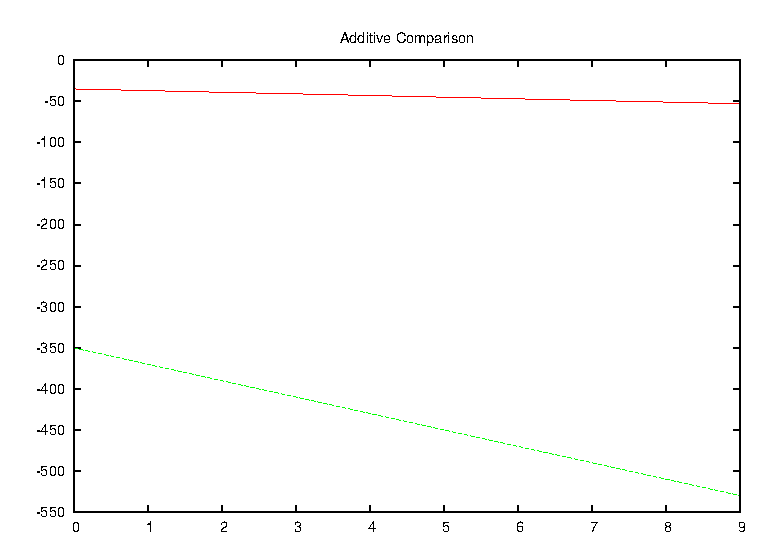
\epsfig{file=data/figures/part1_1,width=8cm,height=6cm}
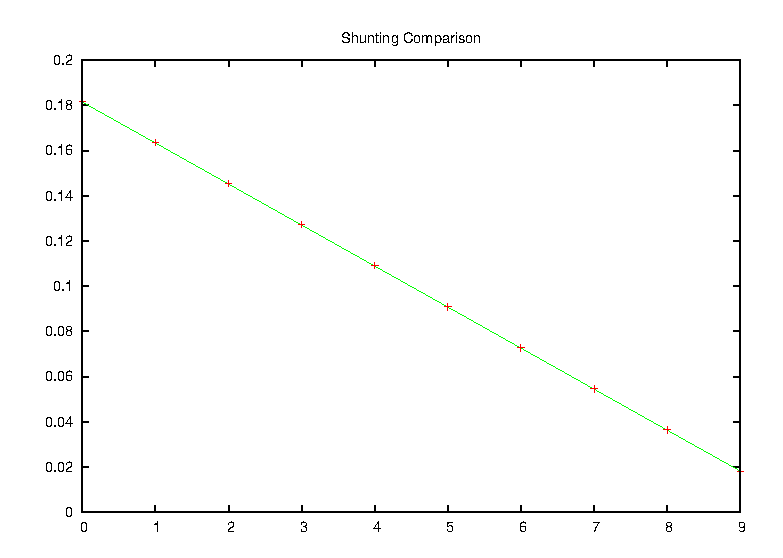
\epsfig{file=data/figures/part1_2,width=8cm,height=6cm}
\end{figure}

\begin{figure}[h!]
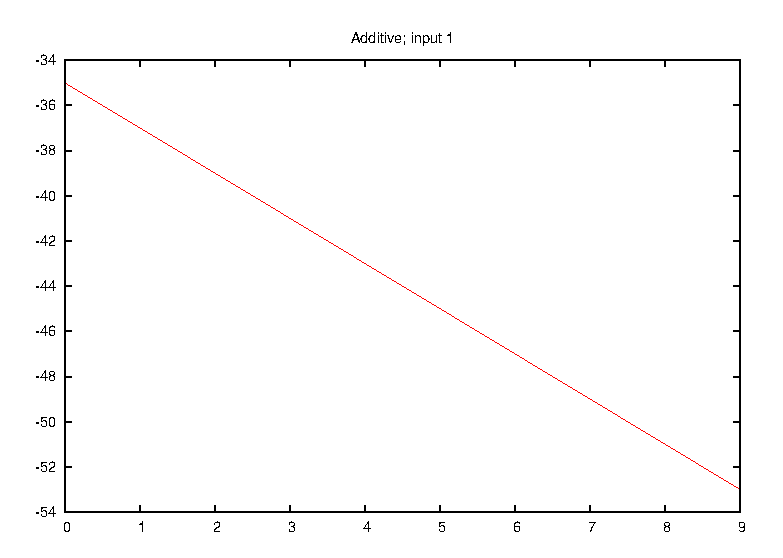
\epsfig{file=data/figures/part1_3,width=8cm,height=6cm}
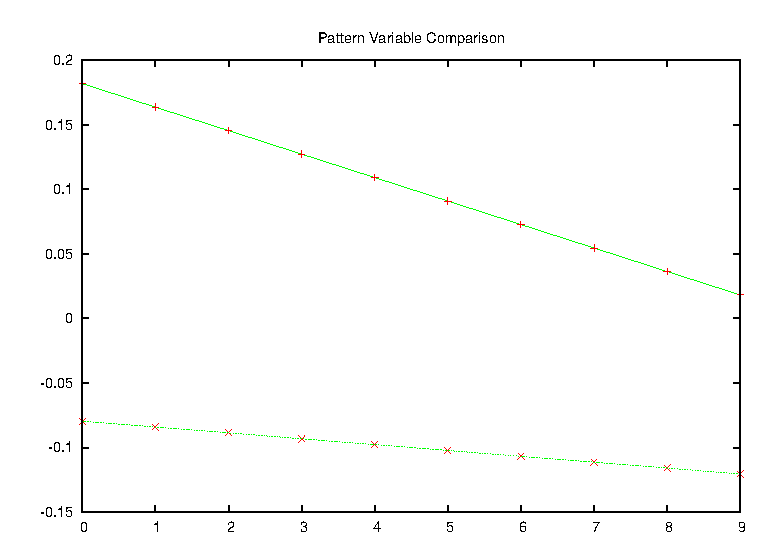
\epsfig{file=data/figures/part1_4,width=8cm,height=6cm}
\end{figure}

The top two graphs show current comparisons for the Additive (left) and Shunting (right) neural networks; the proportionality between current and potential in the Additive network directly reflects the tenfold increase. 

\vspace{2mm}

The bottom left shows the Additive network with the first current configuration (so it could be seen clearly), and the bottom right image shows the comparison of pattern variables for all four tests. 

\vspace{2mm}

The two plots on the right actually show both input currents overlaid on one another; the negation of the overwhelming difference seen previously in the Additive network shows the impact of the pattern variable, though I had some concern with sign (my values should range [-1:1], not [0:1]). 

{\bf Part 2 : Computational Simulation of a Distance-Dependent Shunting network}
\bigskip

Part two of the assignment asks us to simulate a network of 100 neurons using the Distance-Dependent Shunting model. The model contains both excitatory and inhibitory terms which are weighted by the ``distance'' from one neuron to the others; in our case, the distance is quantified by the neuron's index within the network, ranging from 0 to 100. 

\begin{equation}
  \frac{dx_i}{dt} = -Ax_i+(B-x_i)\sum\limits_{k \in D}D_{ki}I_k - (C+x_i)\sum\limits_{l\in E}E_{li}I_l
\end{equation}

Like our other models, this equation can be analytically solved by combining homogeneous and non-homogeneous terms:

\begin{equation}
a=A+\sum\limits_{k \in D}D_{ki}I_k+\sum\limits_{l\in E}E_{li}I_l
\end{equation}
\begin{equation}
b=B\sum\limits_{k \in D}D_{ki}I_k - C\sum\limits_{l\in E}E_{li}I_l
\end{equation}

\begin{equation}
x(t) = Ce^{-at}+b
\end{equation}

The equilibrium solution is then

\begin{equation}
x_i=\frac{B\sum\limits_{k \in D}D_{ki}I_k - C\sum\limits_{l\in E}E_{li}I_l}{A+\sum\limits_{k \in D}D_{ki}I_k+\sum\limits_{l\in E}E_{li}I_l}
\end{equation}

I chose to model this network with wrap-around boundary conditions, meaning neurons close to the end of our index are treated as neighbors to those at the beginning. This effects the value of our sum terms, but the means of solving the equation remain unchanged. These sum terms are weighted by the ``distance'' of a neuron to its neighbors. 

\begin{equation}
D_{ki} = e^{-\frac{(k-i)^2}{F^2}}
\end{equation}
\begin{equation}
E_{li} = 0.5e^{-\frac{(l-i)^2}{G^2}}
\end{equation}

where $F$ and $G$ are weighting parameters. We  throw away any weights less than 0.01, leaving us with a ``radius'' of neighbor neurons which will impact our neuron of interest; 

\begin{equation}
r_D=\sqrt{-F^2ln(0.01)}
\end{equation}

\begin{equation}
r_E=\sqrt{-G^2ln(0.02)}
\end{equation}

This radius is an integer value, and any neurons outside of it (meaning outside of $i \pm R$ can be ignored in our sum.) 

\vspace{2mm}

We simulate this equation for four different input current schemes and two different weighting parameters for a total of eight plots. The equilibrium values were calculated by simulating the distance-dependent shunting equation for a reasonably large period of time; with a time step of 0.05 seconds and a maximum time of 100 seconds, there are a total of 2000 integration steps. 

\vspace{2mm}

The simulation our 1-d network was carried out using the RK4 approximation, which I've simply adapted to a general form and will probably paste around in future assignments. 

\vspace{2mm}

Changing the number of neurons and maximum time have impacts on the runtime; in serial I measured a 2.39s runtime for a $tMax=10,000$ with $n=100$ neurons. The problem at hand is quite parallelizable, however, and most of the computation time is due to the RK4 simulation. 

\vspace{2mm}

By parallelizing this (using an attached OpenCL kernel) I managed to get a runtime of 0.39s for $tMax=10,000$ and $n=1024$ neurons, which is a huge increase. This increase, however, became negligible for our problem wherein something like $tMax=100$, $n=100$ at 0.2s proved to be more than ample time to let our system approach equilibrium. 

\vspace{2mm}

Below you will find my code for running a Runge-Kutta simulation on all neurons given the input current and parameters. 

\vfil\eject

\begin{verbatim}
void simulate(T A, T B, T C, T F, T G, T *I)
{
  // loop variable and current sums
  int i;
  T Esum, Isum;
  // Our sum-radius (nothing outside of it should be included)
  int rE = sqrt(-F*F*log(0.01));
  int rI = sqrt(-G*G*log(0.02));
  // for all N neurons
  for (i=0;i<N;i++)
    {  
      Esum = 0, Isum = 0;
      int k;
      // Calculate the excitatory and inhibitory sums
      for (k=-rE;k<=rE;k++)
        { 
          int r = (i+k+N)%N;
          T e = -(k/F)*(k/F);
          Esum += I[r]*exp(e);
        }
      // Note the wrap around (modulus %) condition
      for (k=-rI;k<=rI;k++)
        { 
          int r = (i+k+N)%N;
          T e = -(k/G)*(k/G);
          Isum += 0.5*I[r]*exp(e);
        }
      // Find equilibrium values over a long period of time
      T x=0,t=0;
      // I can't explain the /100, other than numerical error, but
      // EQ values should still be the same
      T a = (-A-Esum-Isum)/100;
      T b = (B*Esum-C*Isum)/100;
      do {
         x=solveRK(x,a,b);
         t+=DT;
      } while (t<=T_MAX);
      // write data to file
      fprintf(output,"%d\t%lf\n",i+1,x);
    }
}
\end{verbatim}

\vfil\eject

Here we see my solveRK method and eulerAdvance method, as well an OpenCL kernel that could call them once passed in the a and b values of our general form differential equation. 

\begin{verbatim}
T solveRK (T x0, T a, T b)
{
  T k1,k2,k3,k4,s;
  k1 = a*x0+b;
  k2 = a*eulerAdvance(x0,k1,DT/2)+b;
  k3 = a*eulerAdvance(x0,k2,DT/2)+b;
  k4 = a*eulerAdvance(x0,k3,DT)+b;
  s = (k1+2*k2+2*k3+k4);
  return eulerAdvance(x0,s,DT/6.0);
}

T eulerAdvance(T x0, T v, T dt)
{
  return x0 + dt * v;
}
\end{verbatim}

\begin{verbatim}
__kernel void solveEQ
(__global const float* a, __global const float* b, __global float* out, int n) 
{
    int i = get_global_id(0);
    if (i >= n)
        return;

    float x = 0.0f;
    float t = 0.0f;
    float ay = a[i];
    float be = b[i];

    while (t<=T_MAX)
    {
       x = solveRK(x,ay,be);
       t+=DT;
     }
     out[i] = x;
}
\end{verbatim}

\vfil\eject

Now we see the plots from this simulation, which vary in input current scheme and parameters F and G. Again, the initial values for $A$, $B$, and $C$ are 1, 10, and 1.5, respectively. 

\vspace{2mm}

The first output plot shows the neuron equilibriums for the following current scheme: 
\begin{figure}[h!]
\begin{center}
\[
 I =
  \begin{cases}
   10 & \text{if } x \in [1:24] \text{ or } [76:100] \\
   80       & \text{if } x \in [25:75]
  \end{cases}
\]
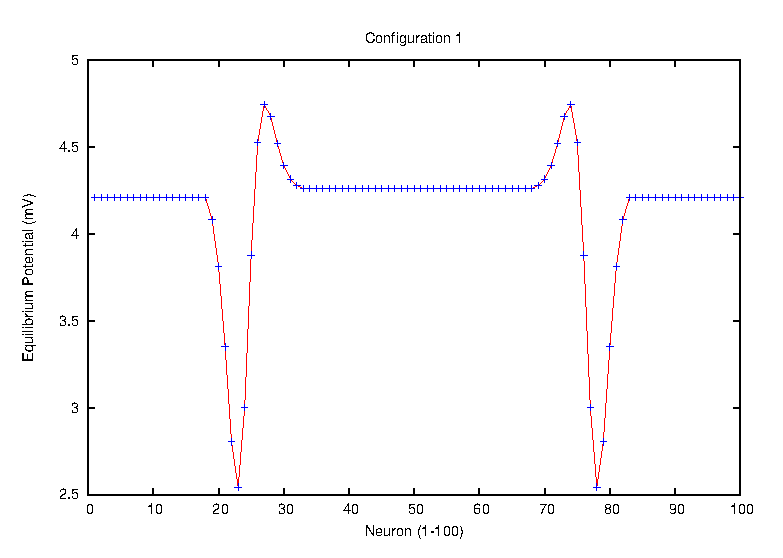
\epsfig{file=data/figures/1,width=15cm,height=10cm}
\end{center}
\caption{\label{pict1}Input Scheme 1, F=2, G=4}

\vspace{2mm}

The first simulation plots an input current that steps from a value of 10 to a value of 80 between neurons 25 $\rightarrow$ 74. Note the effect of neighboring neurons as the current changes from a low to high value.  


\end{figure}

\vfil\eject

\begin{figure}[h!]
\begin{center}
\[
 I =
  \begin{cases}
   10 & \text{if } x \in [1:24] \text{ or } [76:100] \\
   80       & \text{if } x \in [25:75]
  \end{cases}
\]
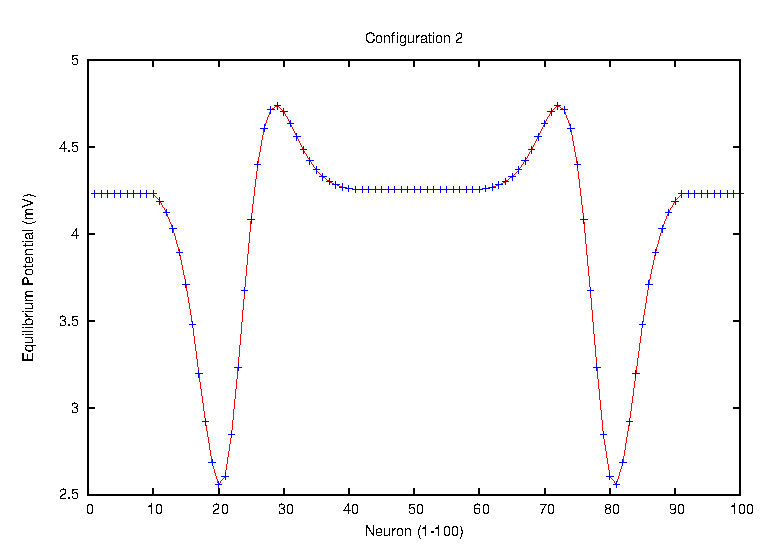
\epsfig{file=data/figures/2,width=15cm,height=10cm}
\end{center}
\caption{\label{pict2}Input Scheme 1, F=4, G=8}

\vspace{2mm}


I noticed that, in general, the increase in F and G (or the ``radius'' of our Gaussian) seemed to smoth out values; I interpreted this smoothness as a supression of inputs whose differences were relatively small, who could have been approximated as being uniform with one another. I think this is what was meant by uniform suppression, though I am not sure. 


\end{figure}
\begin{figure}[h!]
\begin{center}
\[
 I =
  \begin{cases}
   1 & \text{if } x \in [1:24] \text{ or } [76:100] \\
   8       & \text{if } x \in [25:75]
  \end{cases}
\]
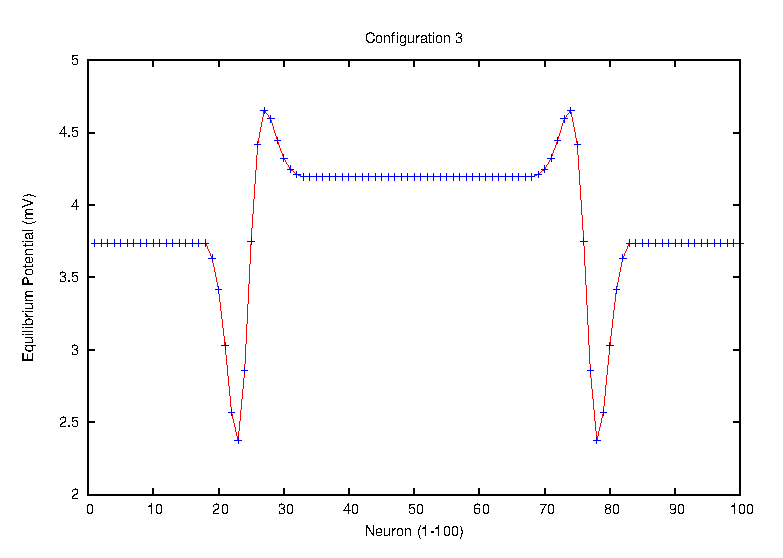
\epsfig{file=data/figures/3,width=15cm,height=10cm}

\vspace{2mm}
\end{center}
\caption{\label{pict3}Input Scheme 2, F=2, G=4}

Since we are using a Distant-Dependent Shunting model, the neurons inhibit one another and generate the same plot as before despite a significantly lower input current. 
\end{figure}

\vfil\eject

\begin{figure}[h!]
\begin{center}
\[
 I =
  \begin{cases}
   1 & \text{if } x \in [1:24] \text{ or } [76:100] \\
   8       & \text{if } x \in [25:75]
  \end{cases}
\]
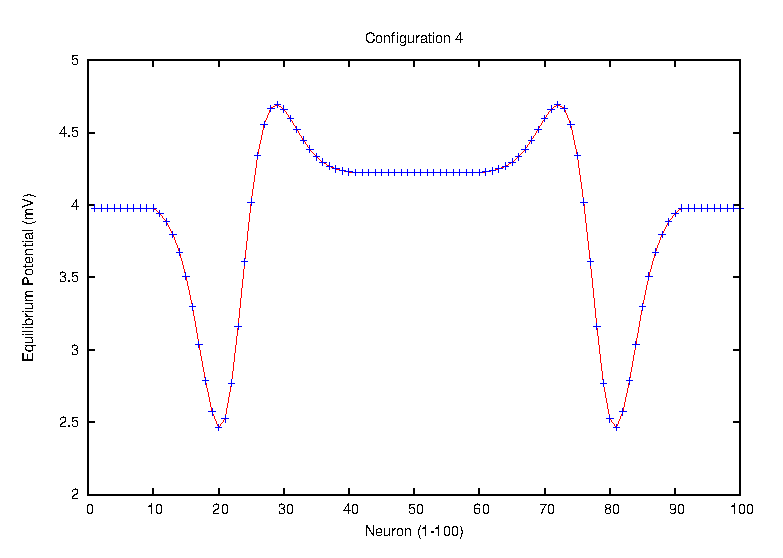
\epsfig{file=data/figures/4,width=15cm,height=10cm}
\end{center}
\caption{\label{pict4}Input Scheme 2, F=4, G=8}

\vspace{2mm}

Similar to before, where an increase in kernel width lead to smoother results. Note the areas of activity occur around changes in input current, and are quick to level off in areas of uniform intensity. 

\end{figure}
\begin{figure}[h!]
\begin{center}
\[
 I =
  \begin{cases}
   10 & \text{if } x \in [1:24] \text{ or } [76:100] \\
   80       & \text{if } x \in [25:75]
  \end{cases}
\]

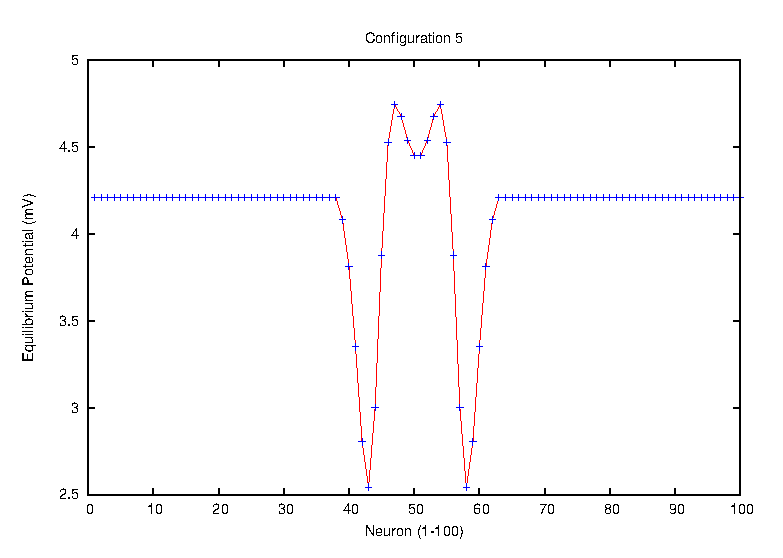
\epsfig{file=data/figures/5,width=15cm,height=10cm}

\end{center}
\caption{\label{pict5}Input Scheme 3, F=2, G=4}

\vspace{2mm}

This was the first of my plots that I think look a bit strange; I'd assume that given the short nature of our current-step we do not allow the neighbors enough space to level off their equilibrium differences. The longer step widths mean that there are fewer areas with high levels of comptetition, and by minimizing this width we can see our radius variable will now have sharper changes to take into account. 

\end{figure}


\vfil\eject

\begin{figure}[h!]
\begin{center}

\[
 I =
  \begin{cases}
   10 & \text{if } x \in [1:44] \text{ or } [56:100] \\
   80       & \text{if } x \in [45:55]
  \end{cases}
\]

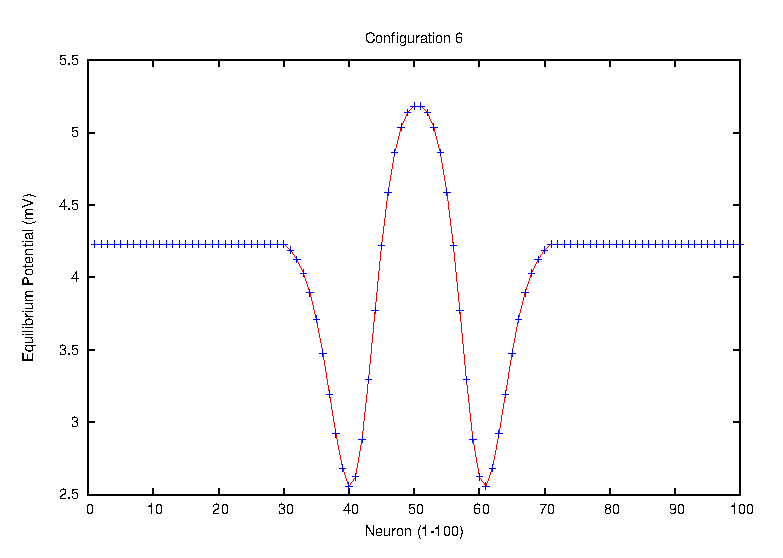
\epsfig{file=data/figures/6,width=15cm,height=10cm}

\end{center}
\caption{\label{pict6}Input Scheme 3, F=4, G=8}


\vspace{2mm}

We see similar behavior here, although the increased kernel width has allowed the middle area to remain smooth. This is an effect of uniform suppression, in which intensities one could see as relatively uniform were approximated as such. 

\end{figure}


\begin{figure}[h!]
\begin{center}

\[
 I =
  \begin{cases}
   1 & \text{if } x \in [1:10] \\
   i - 9 \text{ or } (2 \rightarrow 81) & \text{if } x \in [11:89] \\
   82  & \text{if } x \in [90:100]
  \end{cases}
\]


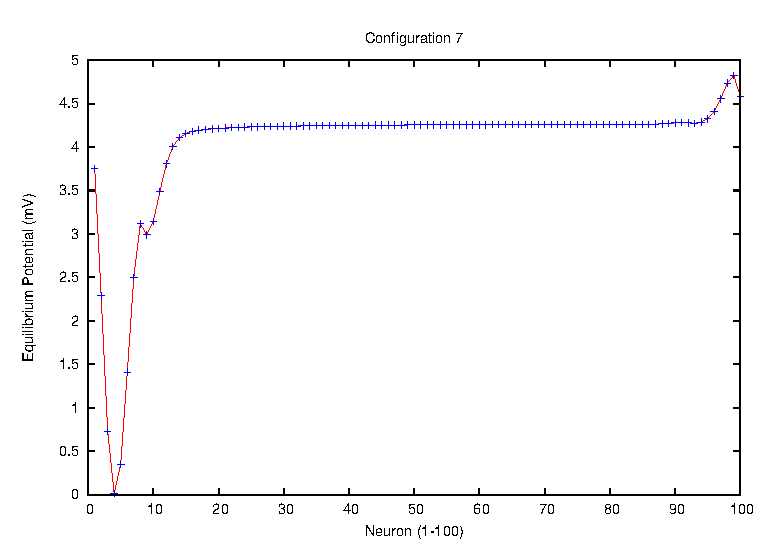
\epsfig{file=data/figures/7,width=15cm,height=10cm}
\end{center}

\caption{\label{pict7}Input Scheme 4, F=2, G=4}

\vspace{2mm}

These may the plots containing ``artifacts'' due to the wrap-around condition. I'm actually not sure what constitutes an artifact, although I assume the sharp changes near the beginning and end of the plot are due to the sharp difference in current intensity between the beginning and end of the network. 

\end{figure}


\begin{figure}[h!]
\begin{center}


\[
 I =
  \begin{cases}
   1 & \text{if } x \in [1:10] \\
   i - 9 \text{ or } (2 \rightarrow 81) & \text{if } x \in [11:89] \\
   82  & \text{if } x \in [90:100]
  \end{cases}
\]


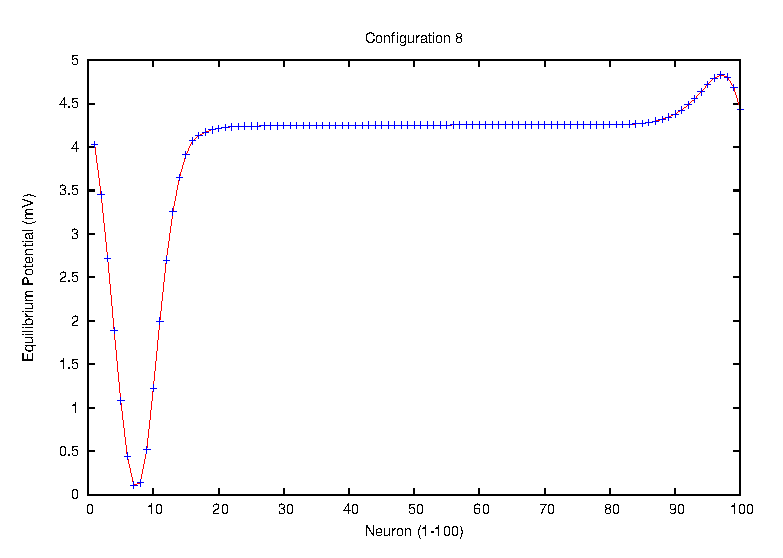
\epsfig{file=data/figures/8,width=15cm,height=10cm}



\end{center}
\caption{\label{pict8}Input Scheme 4, F=4, G=8}

\vspace{2mm}

The smoothing behavior is expected here, and the sharp changes should again be attributed to the wrap-around condition. I suppose if I had padded the edges with their border-value (i.e plenty of 1's toward -x and plenty of 82's toward +x). Still, I would be hesitant to compare this to our initial ramped current, and the difference between the two should be adapted to the distance-dependent nature of the network, in which only local neurons inhibit the neuron at hand. 

\end{figure}

\end{document}
